%-----------------------------------------------------------------------------%
\chapter{\babTiga}
%-----------------------------------------------------------------------------%
Bab ini membahas tentang perancangan dan pemodelan sistem LDPC \textit{codes} DVB-T2 mulai dari \textit{transmitter}, model kanal, hingga \textit{receiver}, juga letak LDPC \textit{codes} dalam sistem tersebut. Bab ini juga mengusulkan \textit{degree distribution} LDPC \textit{codes} DVB-T2, serta teknik untuk menghitung \textit{girth} pada LDPC \textit{codes} dan merancang LDPC \textit{codes} tanpa adanya \textit{girth} 4.
%alir dan model sistem mulai dari \textit{transmitter}, model kanal, hingga \textit{receiver}, juga posisi LDPC \textit{codes} dalam sistem tersebut.

\begin{figure}[tb]
%	\hspace{-6cm}
	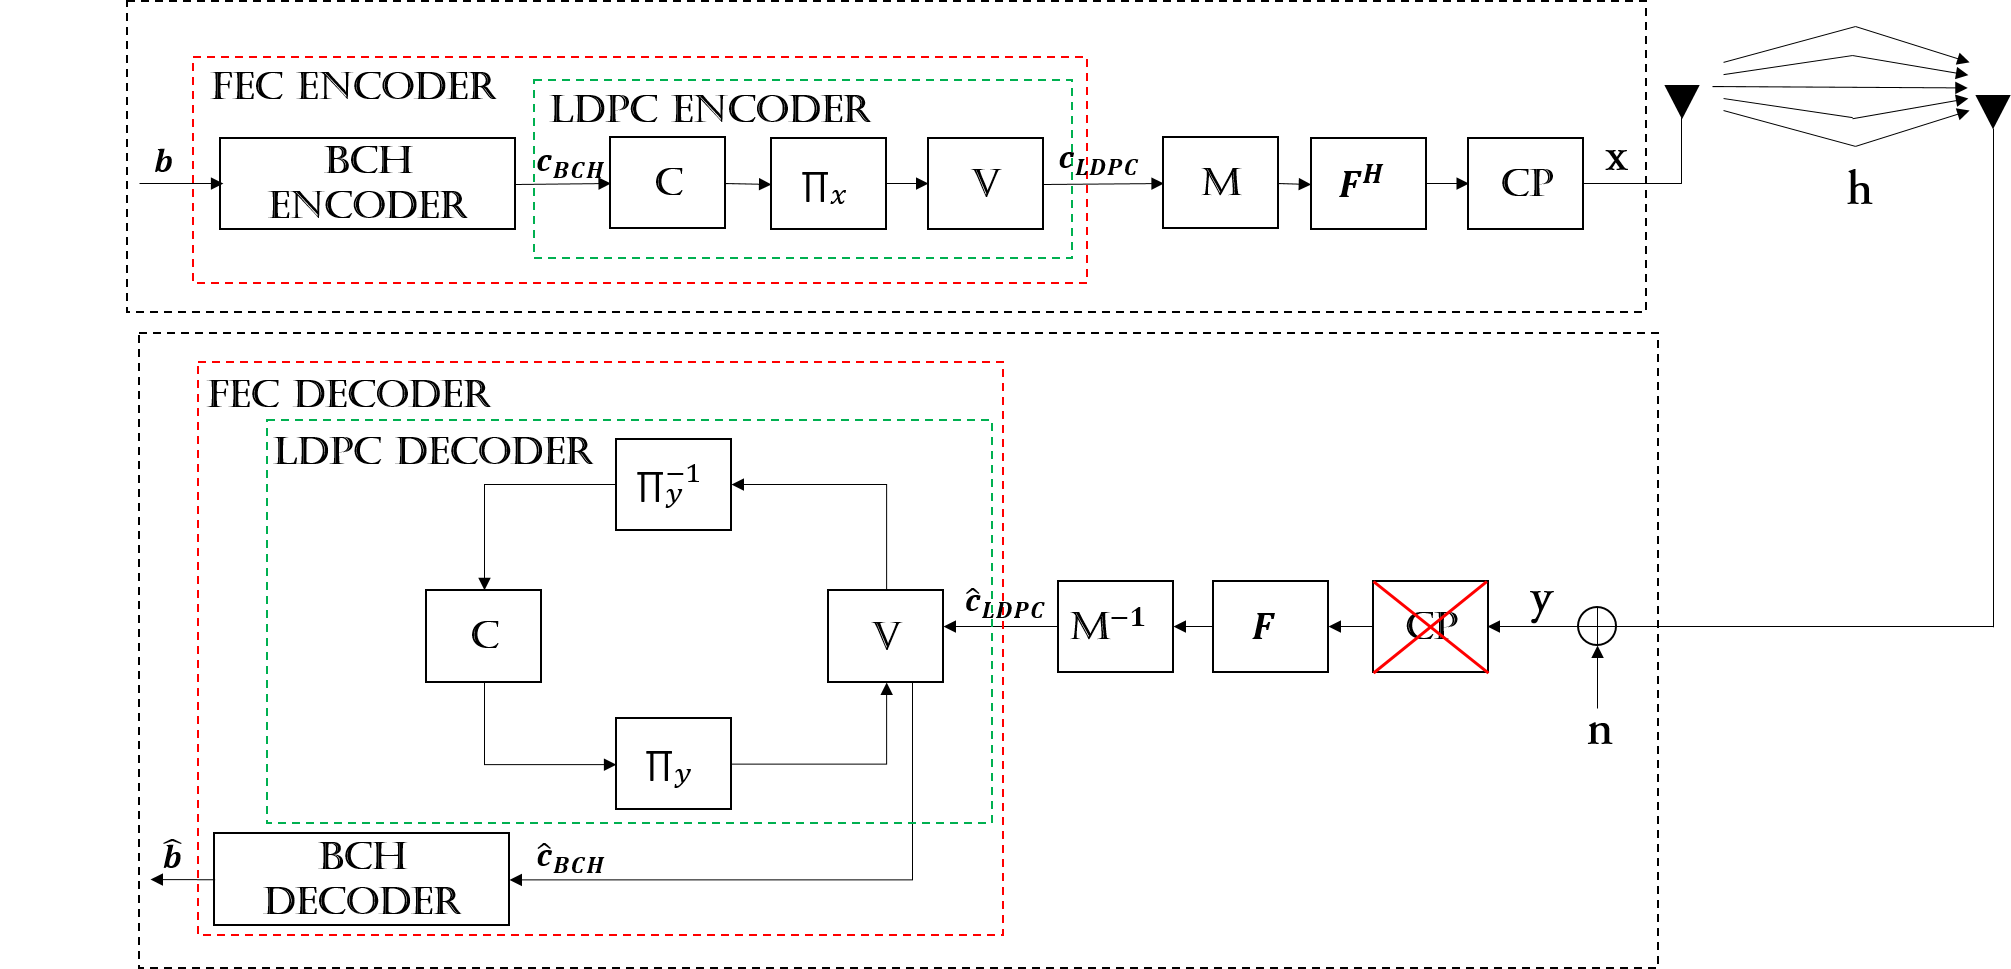
\includegraphics[scale=0.4]
	{pics/sistemmo.png}
	\caption{Diagram blok sistem transmisi DVB-T2 dengan penekanan pada LDPC \textit{codes}.}
	\label{fig:sistem model}
\end{figure}

\begin{figure}[tb]
	\centering
	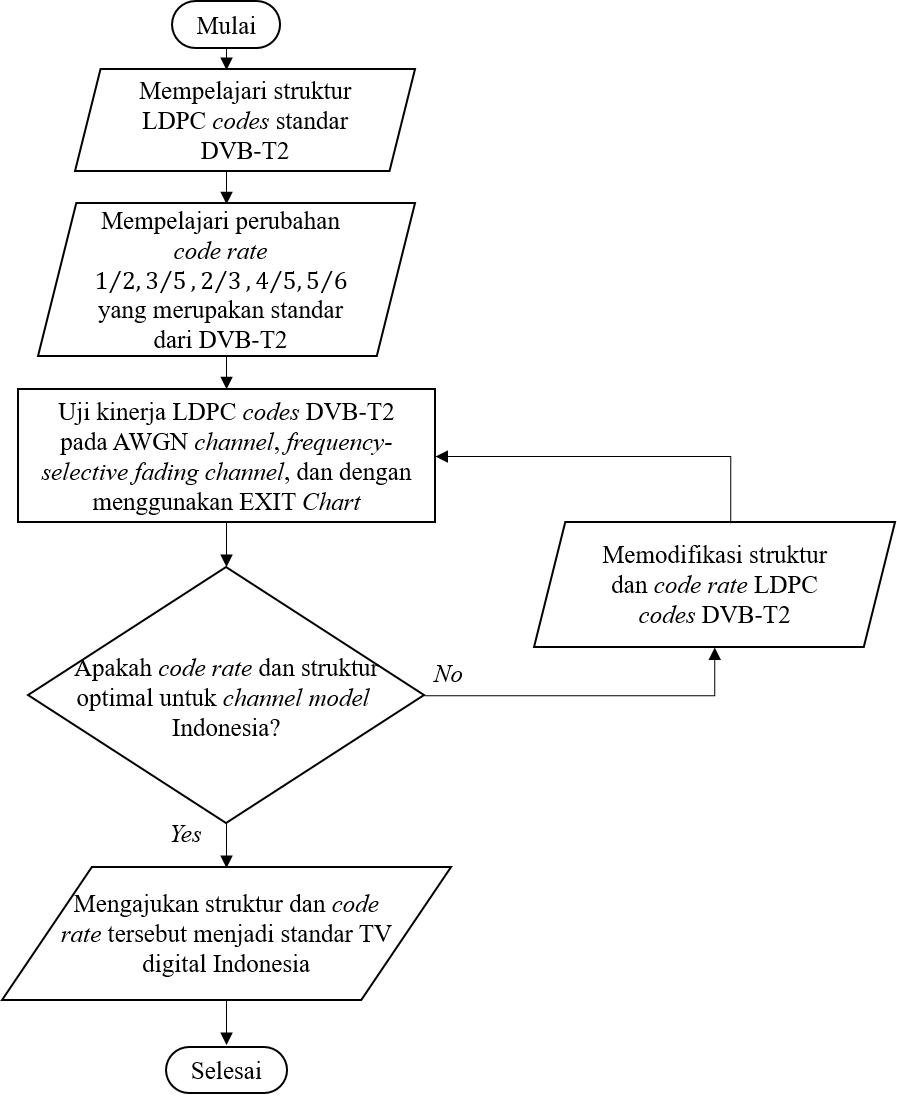
\includegraphics[scale=0.8]
		{pics/diagram/alir.png}
		\caption{Diagram alir evaluasi kinerja LDPC \textit{codes} pada sistem DVB-T2.}
	\label{fig:Diagram Alir}
\end{figure}








%Setelah memahami struktur dari LDPC \textit{codes} DVB-T2, dapat diketahui jika struktur dari LDPC \textit{codes} akan dipengaruhi oleh \textit{code rate} yang digunakan. DVB-T2 memiliki nilai \textit{code rate}: $\frac{1}{2}, \frac{3}{5}, \frac{2}{3}, \frac{3}{4}, \frac{4}{5},$ atau $\frac{5}{6}$ pada standar TS 102 831. Kemudian dilanjutkan dengan mempelajari perubahan yang terjadi dalam penggunaan setiap \textit{code rate} tertenru terhadap struktur dari LDPC \textit{codes}. Berikutnya dilakukan pengujian dan pengamatan kinerja LDPC \textit{codes} dari setiap \textit{code rate} dalam sebuah proses pengiriman data yang menggunakan pemodelan kanal AWGN \textit{Channel} dan \textit{frequency selective fading channel}. Pada langkah selanjutnya, menggunakan EXIT \textit{Chart} untuk menganalisis dan mengoptimalisasi kinerja LDPC \textit{codes} DVB-T2. Apabila hasil dari analisis kinerja LDPC \textit{codes} DVB-T2 yang didapat memiliki kinerja optimal di kondisi alam Indonesia, maka struktur dan \textit{code rate} yang didapat akan diajukan menjadi standar TV digital Indonesia. Namun, apabila LDPC \textit{codes} DVB-T2 memiliki kinerja yang tidak optimal di kondisi alam Indonesia, maka langkah selanjutnya perlu memodifikasi struktur dan \textit{code rate} LDPC \textit{codes} DVB-T2 sehingga dapat bekerja dengan baik dan optimal di kondisi alam Indonesia. 
%-----------------------------------------------------------------------------%
\section{Blok Sistem DVB-T2}
%-----------------------------------------------------------------------------%

%C (CND) V (VND) 
Diagram blok sistem pada Gambar \ref{fig:sistem model} menunjukkan sistem DVB-T2 dari \text{pengirim} ($Tx$) hingga ke penerima ($Rx$) yang berfungsi untuk mempermudah dalam menjelaskan alur komunikasi data DVB-T2. Dimulai dari sisi pengirim, bit informasi $\mathbf{b}$ dibangkitkan secara acak dengan probabilitas kemunculan bit 0 dan 1 sama. Bit yang telah dibangkitkan kemudian masuk ke FEC \textit{encoder}, $\mathbf{b}$ yang masuk ke BCH \textit{encoder} merupakan \textit{outer code} FEC DVB-T2. Setelah itu dari proses BCH \textit{encoder} menghasilkan \textit{codeword} BCH ($\mathbf{c}_{BCH}$) dan akan masuk ke LDPC \textit{encoder} yang merupakan \textit{inner code} FEC DVB-T2. Bit akan di-\textit{encode} oleh Blok C ke Blok V dengan Blok $\Pi_{x}$, sehingga menghasilkan \textit{codeword} ($\mathbf{c}_{LDPC}$). 

Blok C merupakan deretan CND dan Blok V merupakan deretan VND. Blok \textit{Bit Interleaver} ($\Pi_{x}$) mengatur ulang bit, sehingga hasil keluaran dapat dibaca dalam siklus bolak-balik. Kemudian, hasil keluaran dipetakan ke modulasi QPSK yang ditunjukkan dengan Blok $M$, sehingga menghasilkan data berupa simbol per-bit. Simbol akan dikirimkan dengan mode transmisi \textit{orthogonal multi-carrier} yang selanjutnya simbol akan ditransformasikan dari domain frekuensi ke domain waktu pada Blok FFT ($F^{H}$). Blok $F^{H}$ juga berfungsi sebagai OFDM \textit{baseband modulator} yang akan memodulasi frekuensi \textit{subcarrier} untuk setiap simbol yang dibangkitkan pada blok ini. Simbol akan ditambahkan CP untuk mempertahankan \text{properti} ortogonalitas sinyal dan mencegah terjadinya ISI dan ICI. Berikutnya, data akan dikirimkan melalui antena dan melewati kanal \textit{multipath}.

Sinyal terima berupa data yang telah terpengaruhi oleh kanal \textit{multipath} dan \textit{noise}. Kemudian, CP pada sinyal OFDM yang diterima akan dilepas dan sinyal terima akan ditransformasikan kembali dari domain waktu ke domain frekuensi di Blok $F$. Lalu, sinyal terima dikembalikan menjadi bit-bit data pada Blok \textit{Demodulator} ($M^{-1}$) menjadi bit $\hat{\mathbf{c}}_{LDPC}$. Bit $\hat{\mathbf{c}}_{LDPC}$ akan di-\textit{decode} oleh LDPC \textit{decoder} di bagian FEC \textit{decoder}. Proses \textit{iterative decoding} di LDPC \textit{decoder} dilakukan oleh Blok $V$, Blok Bit \textit{Deinterleaver} ($\Pi^{-1}_{y}$), Blok $C$, dan Blok $\Pi_{y}$. Proses \textit{decoding} LDPC \textit{codes} menggunakan SPA, sehingga pada Blok $V$ LLR diproses dengan persamaan 
%Nilai $d_{v}$ adalah jumlah banyak node yang terhubung ke VND,  
\begin{equation}
L_{E_{{v_{i}}}}(n)=L_{ch}+\sum_{j=1,j\neq i}^{d_{v_{n}}} L_{A_{v_{j}}},
\end{equation}
dan pada Blok $C$ 
\begin{equation}
L_{E_{{c_{j}}}}(k)=\sum_{i=1,i\neq j}^{d_{c_{k}}} \boxplus L_{A_{c_{i}}},
\end{equation}
\begin{gather}
L_{E_{c_{j}}}(k)=\sum_{i=1,i\neq j}^{d_{c_{k}}}\boxplus L_{A_{c_{i}}},\\
\approx  (-1) sgn \left \{  L_{A_{c_{i}}} \right \} sgn \left \{ L_{A_{c_{i+1}}} \right \} \cdot \min \left \{ \left | L_{A_{c_{i}}} \right |,\left | 
L_{A_{c_{i+1}}} \right | \right \}.
\end{gather}
%dengan $\Lambda (\theta_{1} ) \boxplus \Lambda (\theta_{2} )$ adalah  
%\begin{eqnarray}
%\Lambda (\theta_{1} ) \boxplus \Lambda (\theta_{2} ) = \ln\frac{e^{\Lambda (\theta _{1})}+e^{\Lambda (\theta _{2})}}{1+e^{\Lambda(\theta_{1})}e^{\Lambda(\theta_{2})}}, \\
%\approx (-1) \mathrm{sgn}\left \{ \Lambda(\theta_{1}) \right \} \mathrm{sgn} \left \{ \Lambda(\theta_{2}) \right \}\cdot \mathrm{min} \left \{ \left | \Lambda(\theta_{1})  \right |, \left | \Lambda(\theta_{2})  \right | \right \}.
%\end{eqnarray}
Setelah proses LDPC \textit{decoding} yang menghasilkan \textit{codeword} BCH \textit{codes} ($\hat{\mathbf{c}}_{BCH}$), $\hat{\mathbf{c}}_{BCH}$ akan masuk ke BCH \textit{decoder} untuk menghasilkan bit informasi ($\hat{\mathbf{b}}$). Bit informasi yang diterima akan dibandingkan dengan bit kirim untuk dianalisis.

\section{Skenario Pengujian Kinerja LDPC \textit{Codes} DVB-T2}
Setiap LDPC \textit{codes} yang terbentuk dari setiap nilai \textit{code rate} akan diuji kinerja BER-nya dan akan dioptimalisasi dengan EXIT \textit{chart} untuk mendapatkan \textit{code rate} dan struktur  LDPC \textit{codes} sehingga dapat bekerja optimal di \textit{channel model} DVB-T2 Indonesia. Apabila kinerja LDPC \textit{codes} dari standar DVB-T2 memiliki kinerja optimal di \textit{channel model} DVB-T2 Indonesia, maka struktur dan \textit{code rate} yang didapat akan diajukan menjadi standar TV digital Indonesia. Namun, apabila LDPC \textit{codes} dari standar DVB-T2 memiliki kinerja yang tidak optimal di \textit{channel model} DVB-T2 Indonesia, maka langkah selanjutnya perlu memodifikasi struktur dan \textit{code rate} LDPC \textit{codes} DVB-T2, sehingga dapat bekerja dengan baik dan optimal pada \textit{channel model} DVB-T2 Indonesia. 
%-----------------------------------------------------------------------------%
%\section{Skenario Pengujian Sistem}
%-----------------------------------------------------------------------------%
%Merujuk ke Tobias Oetiker \cite{tobi_latex}, Tex adalah sebuah program komputer yang dibuat oleh Donald E. Knuth.
%Pengujian sistem dimulai dengan  mempelajari dan memahami struktur standar LDPC \textit{codes} DVB-T2 yang ditunjukkan pada Gambar \ref{fig:Diagram Alir}. 
%\section{Struktur LDPC \textit{Codes} Standar DVB-T2}
%Sesuai standar, DVB-T2 memiliki dua \textit{channel coding}. LDPC \textit{codes} adalah salah satu \textit{channel coding} yang digunakan sebagai \textit{inner codes} dalam FEC DVB-T2. LDPC \textit{codes} DVB-T2 merupakan \textit{irregular} LDPC \textit{codes}. DVB-T2 memiliki panjang blok 16200 dan 64800. DVB-T2 memiliki \textit{parity check} yang pada bagian informasi menggunakan \textit{cyclic structure} dan di bagian \textit{parity}-nya menggunakan \textit{staircase structure}. 
\section{Perancangan LDPC \textit{Codes} DVB-T2}
LDPC \textit{codes} DVB-T2 dengan panjang blok $N_{LDPC}=16200$ memiliki nilai \textit{code rate} $R_e=\left \{ \frac{4}{9}, \frac{3}{5}, \frac{2}{3}, \frac{11}{15}, \frac{7}{9}, \frac{37}{45} \right \}$. Setiap \textit{code rate} pada LDPC \textit{codes} DVB-T2 memiliki nilai \textit{effective code rate} dan VND untuk setiap \textit{variable nodes} yang telah ditunjukkan oleh Tabel \ref{table:dvb-t2lite}. Perancangan matriks \textit{parity check} LDPC \textit{codes} $\mathbf{H}$ untuk setiap \textit{code rate} menggunakan nilai seperti pada Tabel \ref{table:adressldpc}, sedangkan matriks generator $\mathbf{G}$ dibentuk menggunakan Gauss Jordan \textit{elimination}. Tugas Akhir ini melakukan perancangan LDPC \textit{codes} untuk semua \textit{code rate}. 

Matriks $\mathbf{H}$ yang terbentuk pada LDPC \textit{codes} DVB-T2 dengan $N_{LDPC}=16200$ memenuhi dimensi matriks
\begin{equation}
	(1-R_e) \cdot 16200 \times 16200
\end{equation}
dengan $R$ adalah \textit{code rate}, sehingga setiap \textit{code rate} akan mengirimkan bit informasi ($\mathbf{b}$) sebanyak 
\begin{equation}
	b = R_e \times 16200.
\end{equation}

\section{\textit{Quadrature Phase Shift Keying} (QPSK)}
Dalam standar, DVB-T2 dapat menggunakan modulasi QPSK, 16-QAM, 64-QAM, ataupun 256-QAM. Dalam Tugas Akhir ini DVB-T2 menggunakan modulasi QPSK. QPSK memiliki empat kemungkinan simbol. Setiap simbolnya akan membawa dua bit. Setiap fasa dari QPSK memiliki empat kemungkinan dengan nilai 
\begin{equation}
\varphi (t)=(2i-1)\frac{\pi}{4} \;\;\;\;\;\;\;\;\; i=1,2,3,4, 
\label{eq:fasa QPSK}
\end{equation} 
maka setiap simbolnya memiliki persamaan sebagai berikut: 
\begin{equation}
s_{i}(t)=\sqrt{\frac{2E}{T}}cos\left [ (2i-1)\frac{\pi}{4}\right ] cos\left [ 2\pi f_{c}t \right ]-\sqrt{\frac{2E}{T}}sin\left [ (2i-1)\frac{\pi}{4}\right ]sin\left [ 2\pi f_{c}t \right ]
\label{eq:simbol QPSK}
\end{equation}
dengan $0\leq t\leq T$ dan $i=\{ 1\dots 4 \} $. Setiap simbol memiliki nilai fasa yang ditunjukkan pada Tabel \ref{tab:QPSK}.
\begin{table}
	\centering
	\caption{Pemetaan simbol QPSK yang dipakai dalam Tugas Akhir ini.}
	\begin{tabular}{|c|c|lll}
		\cline{1-2}
		Bit informasi & Simbol QPSK \\ \cline{1-2}
		00            &   $\frac{\pi}{4}$  \\ \cline{1-2}
		10            &   $\frac{3\pi}{4}$  \\ \cline{1-2}
		11            &   $\frac{5\pi}{4}$   \\ \cline{1-2}
		01            &   $\frac{7\pi}{4}$    \\ \cline{1-2}
	\end{tabular}
	\label{tab:QPSK}
\end{table}


%DVB-T2 dapat memiliki nilai \textit{code rate}: $\frac{1}{2}, \frac{3}{5}, \frac{2}{3}, \frac{3}{4}, \frac{4}{5},$ atau $\frac{5}{6}$. Nilai-nilai \textit{code rate} tersebut telah ditetapkan oleh standar TS 102.831. Setiap nilai \textit{code rate} akan mempengaruhi bentuk dari LDPC \textit{codes}. Nilai \textit{code rate} terkecil atau $\frac{1}{2}$ memiliki perlindungan proteksi maksimal dan laju data minimal, sedangkan untuk \textit{code rate} terbesar atau $\frac{5}{6}$ memiliki perlindungan proteksi minimal dan laju data maksimal. Dapat diketahui bahwa jika kanal sempurna, maka semakin besar nilai \textit{code rate} akan memiliki laju data yang semakin cepat. Nilai \textit{code rate} sendiri didapatkan dari berbandingan matriks bagian informasi dengan total matriks, sehingga nilai \textit{code rate} akan mempengaruhi matriks LDPC \textit{codes}. Matriks LDPC \textit{codes} terdiri dari bagian informasi dan \textit{parity}, besar keduanya dipengaruhi oleh nilai \textit{code rate} dari LDPC \textit{codes}. 
%\section{Pemodelan Kanal}
%LDPC \textit{codes} akan diuji pada AWGN \textit{channel} dan \textit{frequency selective fading channel} dengan menggunakan \textit{channel model} DVB-T2 di wilayah Indonesia.
%Kondisi probabilitas bersyarat pada sinyal terima, jika yang dikirimkan adalah QPSK
%\begin{equation}
%p(r_{x}\mid t_{x}=+1)=\frac{1}{\sigma \sqrt{2\pi}}\cdot \exp \left ( \frac{\left ( y-1 \right )^{2}}{2\sigma ^{2}} \right ),
%\end{equation}
%\begin{equation}
%p(r_{x}\mid t_{x}=-1)=\frac{1}{\sigma \sqrt{2\pi}}\cdot \exp \left ( \frac{\left ( y+1 \right )^{2}}{2\sigma ^{2}} \right ).
%\end{equation} 
\section{\textit{Channel Model} DVB-T2 Indonesia }
Tugas Akhir ini mensimulasikan proses transmisi \textit{broadband} pada \textit{channel model} DVB-T2 Indonesia berdasarkan \cite{pdpband}, \textit{channel model} DVB-T2 di daerah Bandung digunakan sebagai representasi dari Indonesia.  PDP didapatkan melalui New York \textit{channel simulator} (NYUSIM) dengan menggunakan parameter dari Kota Bandung dan DVB-T2. \textit{Channel model} DVB-T2 pada daerah Bandung mengalamai \textit{frequency selective fading channel}, kondisi yang terjadi saat \textit{bandwidth} kanal lebih kecil daripada \textit{bandwidth} sinyal transmisi. Akibatnya kanal akan mengalami \textit{multipath} dan ISI. Setelah proses normalisasi \textit{channel model} DVB-T2 Bandung menghasilkan \textit{path} sebanyak 8 \textit{path} melalaui NYUSIM. Untuk mengurangi efek dari \textit{frequency selective fading channel} dan \textit{multipath}, DVB-T2 menggunakan OFDM.


\section{\textit{Soft Decoding}}
\textit{Soft decoding} menggunakan \textit{Log-Likehood Ratio} (LLR), LLR merupakan pengukuran statistik untuk membandingkan dua model statistik. LLR membandingkan antar probabilitas pada $p(v)=0$ dan $p(v)=1$. LLR pada sinyal terima $y$ dapat dihitung dengan
\begin{eqnarray}
LLR &=& \log\frac{P\left ( y\mid x=+1 \right )}{P\left ( y\mid x=-1   \right )}, \nonumber \\
LLR &=& \frac{2}{\sigma ^2}\cdot y
\end{eqnarray}
dengan $\sigma$ adalah variansi untuk \textit{double-sided noise} dengan distribusi Gaussian.
% 
%Tugas Akhir ini mengasumsikan komunikasi nirkabel TV digital dengan transmisi \textit{broadband}, maka dari itu \textit{frequency selective fading channel} diajukan sebagai pemodelan kanalnya. \textit{Frequency selective fading channel} adalah kondisi saat \textit{bandwidth} kanal lebih kecil daripada \textit{bandwidth} sinyal transmisi, akibatnya kanal akan menghasilkan \textit{multipath} dan ISI. Model matematika \textit{frequency selective fading channel} 
%\begin{equation}
%Y(f)=X(f)H(f)+N(f),
%\end{equation}
%dengan $X(f)$ didefinisikan sebagai sinyal yang dikirimkan dalam \textit{domain} frekuensi, $H(f)$ sebagai respon frekuensi dari kanal, $N(f)$ sebagai \textit{noise thermal} yang terdistribusi Gaussian, dan $Y(f)$ sebagai sinyal diterima dalam \textit{domain} frekuensi.  
%\begin{figure}[tb]
%\centering
%	\includegraphics[scale=0.62]
%		{pics/kon.png}
%		\caption{Diagram konstelasi QPSK.}
%	\label{fig:BER}
%\end{figure}



 \begin{figure}[tb]
	
	\centering
	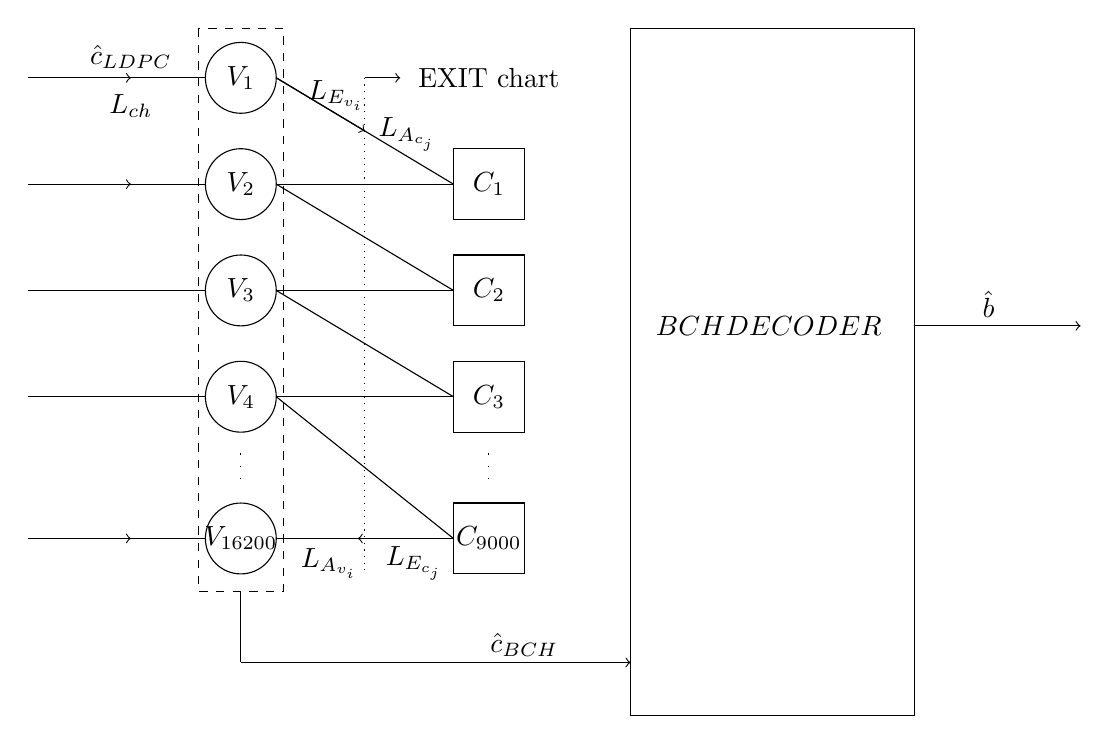
\begin{tikzpicture}[scale=0.9]
	
	\draw (1,-6) -- (2.45,-6)[->];
	\node at (2.45,-5.7) {$\hat{c}_{LDPC}$};
	\node at (2.45,-6.4) {$L_{ch}$};
	
	\draw (1,-6) -- (3.5,-6);
	\draw (1,-7.5) -- (3.5,-7.5);
	\draw (1,-7.5) -- (2.45,-7.5)[->];
	\node at (5.35,-6.25) {$L_{E_{v_{i}}}$};
	\node at (6.35,-6.8) {$L_{A_{c_{j}}}$};
	
	\draw (1,-9) -- (3.5,-9);
	\draw (1,-10.5) -- (3.5,-10.5);
	\draw (1,-12.5) -- (3.5,-12.5);
	\draw (1,-12.5) -- (2.45,-12.5)[->];
	\node at (5.25,-12.85) {$L_{A_{ v_{i}}}$};
		\node at (6.45,-12.85) {$L_{E_{c_{j}}}$};
	
	
	\draw (7,-8) rectangle (8,-7); \node at (7.5,-7.5) {$C_1$};
	\draw (7,-8.5) rectangle (8,-9.5); \node at (7.5,-9) {$C_2$};
	\draw (7,-10) rectangle (8,-11); \node at (7.5,-10.5) {$C_3$};
	\draw (7.5,-11.3) [loosely dotted]-- (7.5,-11.7);
	\draw (7,-12) rectangle (8,-13); \node at (7.5,-12.5) {$C_{9000}$};
	
	
	\draw (5.75,-6) [dotted]--  (5.75,-13);
	\draw (5.75,-6) --  (6.25,-6)[->];
	\node at (7.5,-6) {EXIT chart};
	
	
	\draw (4,-6) circle [radius=0.5]; \node at (4,-6) {$V_{1}$};
	\draw (4,-7.5) circle [radius=0.5]; \node at (4,-7.5) {$V_{2}$};
	\draw (4,-9) circle [radius=0.5]; \node at (4,-9) {$V_{3}$};
	\draw (4,-10.5) circle [radius=0.5]; \node at (4,-10.5) {$V_{4}$};
	\draw (4,-11.3) [loosely dotted] -- (4,-11.7);
	\draw (4,-12.5) circle [radius=0.5]; \node at (4,-12.5) {$V_{16200}$};
	\draw (3.4,-5.3) [dashed] rectangle (4.6,-13.25);
	\draw (4,-13.25) -- (4,-14.25);
	\draw (4,-14.25) -- (9.5,-14.25) [->];
	\draw (9.5,-5.3)  rectangle (13.5,-15); \node at (11.45,-9.5) {$BCH DECODER$};
	\draw (13.5,-9.5) -- (15.85,-9.5) [->];\node at (14.55,-9.2) {$\hat{b}$}; 
	\node at (8,-14) {$\hat{c}_{BCH}$};
	
	
	\draw (4.5,-6) -- (7,-7.5);
	\draw (4.5,-6) -- (5.75,-6.75)[->];
	
	\draw (4.5,-7.5) -- (7,-7.5);
	\draw (4.5,-7.5) -- (7,-9);
	\draw (4.5,-9) -- (7,-9);
	\draw (4.5,-9) -- (7,-10.5);
	\draw (4.5,-10.5) -- (7,-10.5);
	\draw (4.5,-10.5) -- (7,-12.5);
	\draw (4.5,-12.5) -- (7,-12.5);
	
	\draw (5.65,-12.5) -- (7,-12.5)[<-];
	
	\end{tikzpicture}
	\caption{Representasi Tanner \textit{graph} LDPC \textit{codes} DVB-T2  dengan $N_{LDPC}=16200$ dan \textit{code rate} $R_e=\frac{4}{9}$.}
\label{fig:tannerasli}
\end{figure}



\section{Usulan LDPC \textit{Codes} DVB-T2 dengan $N_{LDPC}=16200$}
LDPC \textit{codes} dibentuk menggunakan Tabel \textit{Addresses Parity Bit Accumulator} berdasarkan standar DVB-T2 untuk LDPC \textit{codes} DVB-T2 dengan panjang $N_{LDPC}=16200$. Tugas Akhir ini menyimbolkan VND $d_v$ pada LDPC \textit{codes} DVB-T2 sebagai $\Lambda (x)$, sedangkan CND $d_c$ disimbolkan sebagai $\Omega(x)$. \textit{Degree distribution} pada \textit{downscaled} LDPC \textit{codes} yang diusulkan oleh Tugas Akhir ini untuk \textit{code rate} $R_e=\frac{4}{9}$ adalah:
\begin{eqnarray}
\Lambda (x) &=& \frac{1}{16200}x+\frac{8999}{16200}x^2+\frac{5400}{16200}x^3+\frac{1800}{16200}x^8, \\
\Omega(x) &=& \frac{1441}{9000}x^4+\frac{3239}{9000}x^5+\frac{3600}{9000}x^6+\frac{720}{9000}x^7,
\end{eqnarray}
dan untuk \textit{code rate} $R_e=\frac{3}{5}$ adalah:
\begin{eqnarray}
\Lambda (x) &=& \frac{1}{16200}x+\frac{6479}{16200}x^2+\frac{6480}{16200}x^3+\frac{3240}{16200}x^{12},   \\
\Omega(x) &=& \frac{1}{6480}x^8+\frac{6479}{6480}x^9,
\end{eqnarray}
dan untuk \textit{code rate} $R_e=\frac{2}{3}$ adalah:
\begin{eqnarray}
\Lambda (x) &=& \frac{1}{16200}x+\frac{5399}{16200}x^2+\frac{9720}{16200}x^3+\frac{1080}{16200}x^{13},   \\
\Omega(x) &=& \frac{1}{5400}x^{9}+\frac{5339}{5400}x^{10},
\end{eqnarray}
dan untuk \textit{code rate} $R_e=\frac{11}{15}$ adalah:
\begin{eqnarray}
\Lambda (x) &=& \frac{1}{16200}x+\frac{4319}{16200}x^2+\frac{11520}{16200}x^3+\frac{360}{16200}x^{12},   \\
\Omega(x) &=& \frac{361}{4320}x^{9}+\frac{1079}{4320}x^{10}+\frac{1440}{4320}x^{11},+\frac{1080}{4320}x^{12}+\frac{360}{4320}x^{13},
\end{eqnarray}
dan untuk \textit{code rate} $R_e=\frac{7}{9}$ adalah:
\begin{eqnarray}
\Lambda (x) &=& \frac{1}{16200}x+\frac{3599}{16200}x^2+\frac{12600}{16200}x^3,   \\
\Omega(x) &=& \frac{361}{3600}x^{11}+\frac{1079}{3600}x^{12}+\frac{2160}{3600}x^{13},
\end{eqnarray}
dan untuk \textit{code rate} $R_e=\frac{37}{45}$ adalah:
\begin{eqnarray}
\Lambda (x) &=& \frac{1}{16200}x+\frac{2879}{16200}x^2+\frac{12960}{16200}x^3 +\frac{360}{16200}x^{13} , \\
\Omega(x) &=& \frac{1}{2880}x^{15}+\frac{1439}{2880}x^{16}+\frac{360}{2880}x^{17}+\frac{360}{2880}x^{18}+\frac{720}{2880}x^{19}.
\end{eqnarray}
\section{Usulan LDPC \textit{Codes} DVB-T2 menggunakan Teknik \textit{Downscaling}}

Teknik \textit{downscaling} digunakan untuk mengurangi kompleksitas komputasi pada \textit{encoder} dan \textit{decoder}, sehingga akan meringankan proses simulasi dan memungkinkan untuk \textit{device} dengan kemampuan komputasi rendah \cite{scale}. Langkah-langkah untuk melakukan \textit{downscaling} LDPC \textit{codes} DVB-T2 adalah sebagai berikut: 

\begin{enumerate}
	\item Tentukan \textit{scaling factor} $s_f$, $s_f$ harus merupakan faktor dari $360$. 
	\item Masukkan nilai pada Tabel \textit{Addresses Parity Bit Accumulator} seperti pada Tabel \ref{table:adressldpc} ke $p_{1}(j), p_{2}(j), p_{3}(j), \dots$$, p_{q}(j)$, $j= 1, 2, 3, \dots, J$  dan $q= 1, 2, 3, \dots, Q$. 
%	$j$ menunjukkan kolom dan  $q$ menunjukkan baris dari Tabel \ref{table:dvb-t2lite}.
	\item Hitung $r_{1}(j), r_{2}(j), r_{3}(j), \dots, r_{q}(j)$
	\begin{equation}
	r_{q}(j)=mod\left \{ \left [ p_q(j) + J \times \left ( k-1 \right ) \right ],\left [ P/s_f \right ] \right \},
	\end{equation}
	\item Nilai $r_q(j)$ akan menjadi Tabel \textit{Addresses Parity Bit Accumulator} baru untuk \textit{downscaled} LDPC \textit{codes} DVB-T2. 
\end{enumerate}
Parameter $q$ adalah kolom dan $j$ adalah baris dari Tabel \textit{Addresses Parity Bit Accumulators}.  Nilai $s_f$ akan menentukan panjang blok matriks \textit{parity check} \textit{downscaled} LDPC \textit{codes} DVB-T2. $P$ adalah nilai dari baris original matriks LDPC \textit{codes} DVB-T2, nilai $k$ memiliki batas dengan $1< k \leq \left ( 360/s_f \right )$. Nilai $360$ adalah jumlah \textit{node indices} LDPC \textit{codes} DVB-T2.


\begin{figure}[b!]
	\centering
	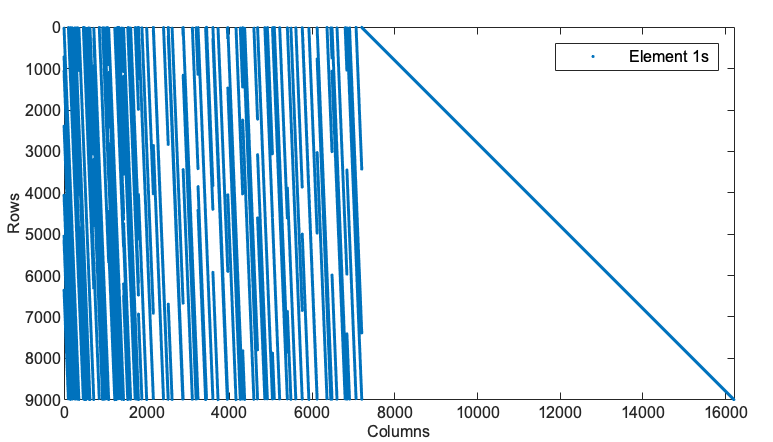
\includegraphics[width=1\textwidth]
	{pics/hs(1-2)-2}
	\caption{Matriks \textit{parity check} original DVB-T2 LDPC \textit{codes} dengan $N_{LDPC}=16200$.}
	\label{fig:hori}
\end{figure}

%\begin{figure}
%	\centering
%%	\hspace{-0.2 in}
%	\begin{minipage}{1\linewidth}
%		\hspace{1.5 cm}
%		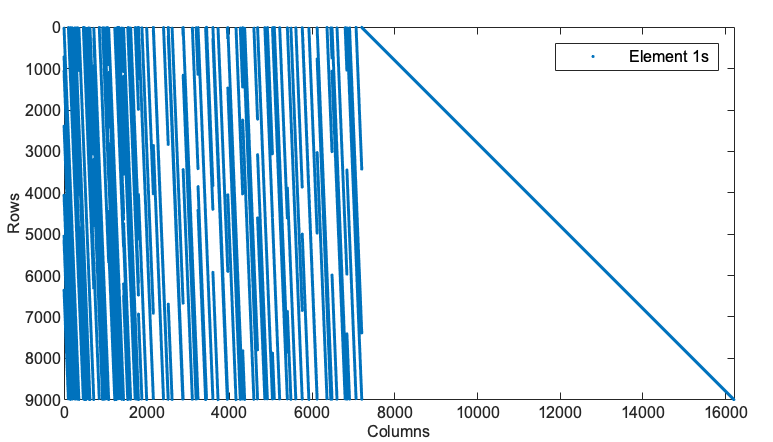
\includegraphics[width=0.9\textwidth]{pics/hs(1-2)-2}
%		\vspace{-0.5cm}
%		
%		\center (a)
%	\end{minipage}
%	\hfill
%%	\hspace{0.05 in}
%	\begin{minipage}{1\linewidth}
%		\hspace{1.5 cm}
%		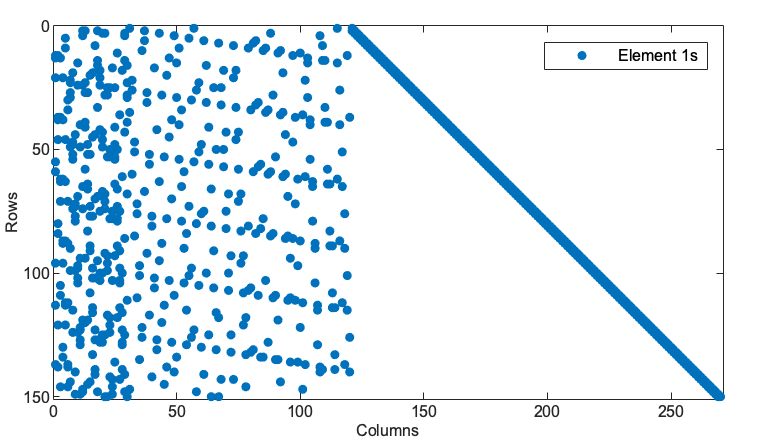
\includegraphics[width=0.9\textwidth]{pics/hs1-60(1-2)-2}
%		\vspace{-0.5cm}
%		\center (b)
%	\end{minipage}
%	\caption {Matriks \textit{parity check} DVB-T2 LDPC \textit{codes} (a) $N_{LDPC}=16200$ dan (b) $N_{LDPC}=270$.}
%	\label{gambar: banding}
%\end{figure}


\begin{figure}[t!]
	\centering
	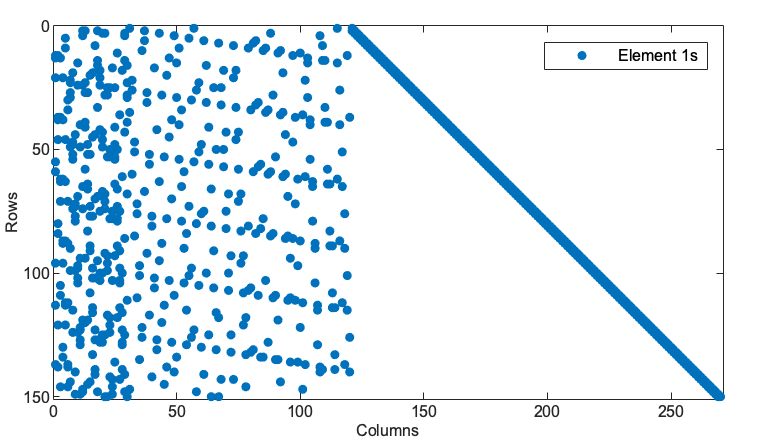
\includegraphics[width=1\textwidth]
	{pics/hs1-60(1-2)-2}
	\caption{Matriks \textit{downscaled} \textit{parity check} DVB-T2 LDPC \textit{codes} dengan $N_{LDPC}=270$.}
	\label{fig:hds}
\end{figure}
%\begin{figure}[tb]
%	\centering 
%
%	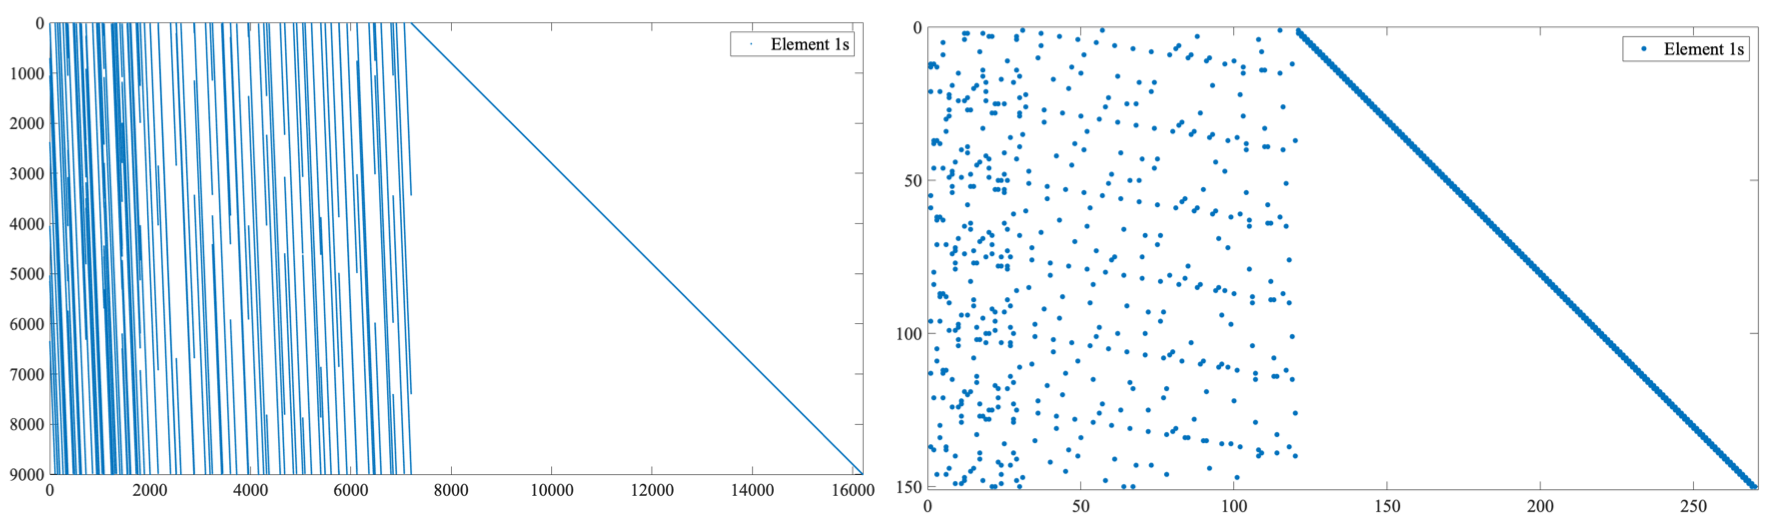
\includegraphics[scale=0.5]{pics/banding}
%	\centering 
%	\caption{Perbandingan matriks \textit{parity check} LDPC \textit{codes} DVB-T2 original dengan \textit{downscaled}.}
%	\label{fig:banding}
%\end{figure}

Tugas Akhir ini menggunakan \textit{scaling factor} $s_f=60$ untuk mengetahui efek \textit{downscaling} pada kinerja LDPC \textit{codes} DVB-T2  dan meringankan proses simulasi. \textit{Downscaled} matriks \textit{parity check}  LDPC \textit{codes} ditunjukkan oleh Gambar  \ref{fig:hds}, sedangkan original matriks \textit{parity check}  LDPC \textit{codes} ditunjukkan oleh Gambar \ref{fig:hori}. Tugas Akhir ini telah melakukan \textit{downscaling} untuk semua \textit{code rate} pada LDPC \textit{codes} DVB-T2, karena $s_f=60$ maka \textit{downscaled} LDPC \textit{codes} DVB-T2 memiliki panjang blok $N_{LDPC}=270$.

Tugas Akhir ini menyimbolkan VND $d_v$ pada LDPC \textit{codes} DVB-T2 sebagai $\Lambda (x)$, sedangkan CND $d_c$ disimbolkan sebagai $\Omega(x)$. \textit{Degree distribution} pada \textit{downscaled} LDPC \textit{codes} yang diusulkan oleh Tugas Akhir ini untuk \textit{code rate} $R_e=\frac{4}{9}$ adalah:
\begin{eqnarray}
\Lambda (x)&=&\frac{1}{270}x+\frac{149}{270}x^2+\frac{90}{270}x^3+\frac{30}{270}x^8, \\
\Omega(x)&=&\frac{25}{150}x^4+\frac{53}{150}x^5+\frac{60}{150}x^6+\frac{12}{150}x^{12},
\end{eqnarray}
untuk \textit{code rate} $R_e=\frac{3}{5}$ adalah:
\begin{eqnarray}
\Lambda (x)&=&\frac{1}{270}x+\frac{107}{270}x^2+\frac{132}{270}x^3+\frac{30}{270}x^{12},\\
\Omega(x)&=&\frac{1}{108}x^8+\frac{107}{108}x^9,
\end{eqnarray}
untuk \textit{code rate} $R_e=\frac{2}{3}$ adalah:
\begin{eqnarray}
\Lambda (x)&=&\frac{1}{270}x+\frac{89}{270}x^{2}+\frac{162}{270}x^{3}+\frac{18}{270}x^{13},\\
\Omega(x)&=&\frac{1}{90}x^{9}+\frac{89}{90}x^{10},
\end{eqnarray}
untuk \textit{code rate} $R_e=\frac{11}{15}$ adalah:
\begin{eqnarray}
\Lambda (x)&=&\frac{1}{270}x+\frac{71}{270}x^{2}+\frac{192}{270}x^{3}+\frac{6}{270}x^{12},\\
\Omega(x)&=&\frac{7}{72}x^{9}+\frac{11}{72}x^{10}+\frac{36}{72}x^{11}+\frac{12}{72}x^{12} \nonumber \\ &&+\frac{6}{72}x^{13}.
\end{eqnarray}
untuk \textit{code rate} $R_e=\frac{7}{9}$ adalah:
\begin{eqnarray}
\Lambda (x)&=&\frac{1}{270}x+\frac{71}{270}x^2+\frac{198}{270}x^3,\\
\Omega(x)&=&\frac{7}{60}x^{11}+\frac{29}{60}x^{12}+\frac{24}{60}x^{13},
\end{eqnarray}
dan untuk \textit{code rate} $R_e=\frac{37}{45}$ adalah:
\begin{eqnarray}
\Lambda (x)&=&\frac{1}{270}x+\frac{71}{270}x^{2}+\frac{192}{270}x^{3}+\frac{6}{270}x^{12},\\
\Omega(x)&=&\frac{7}{48}x^{15}+\frac{17}{48}x^{16}+\frac{18}{48}x^{17}+\frac{6}{48}x^{18},
\end{eqnarray}
\textit{Degree distribution} untuk setiap \textit{code rate} tetap memenuhi ketentuan pada Tabel \ref{table:dvb-t2lite} dengan jumlah yang disesuaikan pada ukuran matriksnya.

\section{Usulan Algoritma PEG}
Tugas Akhir ini mengusulkan Algoritma PEG menggunakan metode kedua dari PEG yaitu dengan memilih nilai CND terkecil secara terurut. Pada langkah kedua PEG, Tugas Akhir ini menambahkan sebuah algoritma untuk menghindari pembentukkan LDPC \textit{codes} dengan \textit{girth}-4 yang dinamakan algoritma \textit{Anti Girth}-4. Penggunaan PEG dalam pembuatan matriks \textit{parity check} LDPC \textit{codes} memungkinkan untuk membuat matriks \textit{parity check} LDPC \textit{codes} sesuai dengan nilai panjang blok $n$, baris $m$, dan set dari VND~$D_v=\{ d_{v_1}, d_{v_2}, d_{v_3}, \cdots ,d_{v_n} \}$ yang telah ditentukan. Proses penempatan elemen 1 dimulai dari kolom 1 sampai $n$ dan dari baris 1 ke $m$ yang prosesnya berjalan dari kiri ke kanan dan dari atas ke bawah.

\subsection{Langkah PEG}
Langkah-langkah perancangan matriks \textit{parity check} LDPC \textit{codes} menggunakan algoritma PEG yang diusulkan dengan nilai $n=8$, $m=5$, dan $D_v=\{ 2, 2, 2, 2 ,2 \}$ adalah sebagai berikut:
%\begin{equation}
%%\begin{figure}
%%	\centering 
%%		\hspace{0.75cm}
%%	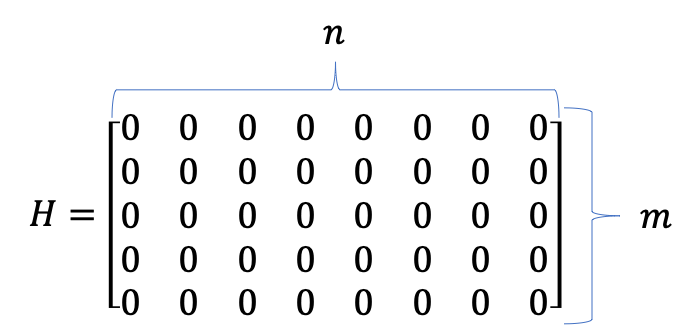
\includegraphics[scale=0.5]{pics/step1}
%%	\centering 
%\mathbf{B}_r=
%\begin{tikzpicture}[baseline=-\the\dimexpr\fontdimen22\textfont2\relax ]
%\matrix (m)[matrix of math nodes,left delimiter=(,right delimiter=)]
%{
%	0 & 0 & 1 & 0 \\
%	1 & 0 & 1 & 0 \\
%	1 & 0 & 1 & 1 \\
%	0 & 1 & 0 & 1 \\
%};
%\begin{pgfonlayer}{myback}
%\fhighlight[green!30]{m-1-3}{m-4-3}
%\end{pgfonlayer}
%\end{tikzpicture}
%
%%\end{figure}
%\end{equation}


\begin{equation}
\mathbf{H}=
\begin{tikzpicture}[baseline=-\the\dimexpr\fontdimen22\textfont2\relax ]
\matrix (m)[matrix of math nodes,left delimiter=(,right delimiter=)]
{
	0 & 0 & 0 & 0 & 0 & 0 & 0 & 0\\
	0 & 0 & 0 & 0 & 0 & 0 & 0 & 0\\
	0 & 0 & 0 & 0 & 0 & 0 & 0 & 0\\
	0 & 0 & 0 & 0 & 0 & 0 & 0 & 0\\
	0 & 0 & 0 & 0 & 0 & 0 & 0 & 0 \\
};
\begin{pgfonlayer}{myback}
%\fhighlight[green!30]{m-1-3}{m-4-3}
\end{pgfonlayer}
\end{tikzpicture}
\end{equation}

\begin{itemize}
	\item[1.] Buat matriks nol dengan dimensi $m\times n$, dengan $n$ adalah jumlah variable \textit{nodes} dan $m$ adalah jumlah \textit{check nodes} yang telah ditentukan.
\end{itemize}
%\begin{figure}
%	\centering 
%	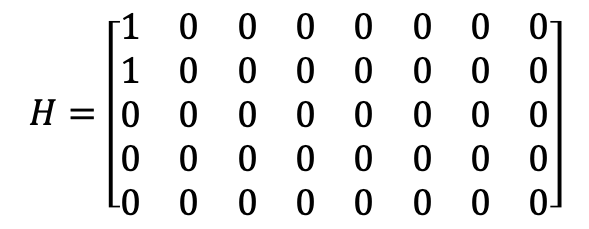
\includegraphics[scale=0.5]{pics/step2}
%	\centering 
%\end{figure}
\begin{equation}
\mathbf{H}=
\begin{tikzpicture}[baseline=-\the\dimexpr\fontdimen22\textfont2\relax ]
\matrix (m)[matrix of math nodes,left delimiter=(,right delimiter=)]
{
	1 & 0 & 0 & 0 & 0 & 0 & 0 & 0\\
	1 & 0 & 0 & 0 & 0 & 0 & 0 & 0\\
	0 & 0 & 0 & 0 & 0 & 0 & 0 & 0\\
	0 & 0 & 0 & 0 & 0 & 0 & 0 & 0\\
	0 & 0 & 0 & 0 & 0 & 0 & 0 & 0 \\
};
\begin{pgfonlayer}{myback}
%\fhighlight[green!30]{m-1-3}{m-4-3}
\end{pgfonlayer}
\end{tikzpicture}
\end{equation}
\begin{itemize}
	\item[2.] Elemen 1 pertama ditempatkan sesuai dengan algoritma pertama dari proses PEG. Elemen 1 kedua dan seterusnya sebanyak $d_v(n)$ ditempatkan menggunakan kombinasi algoritma PEG dengan \textit{Anti Girth}-4.
\end{itemize}
%\begin{figure}
%	\centering 
%	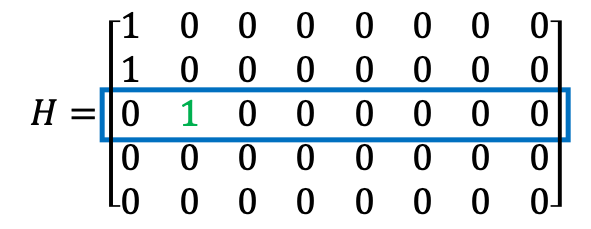
\includegraphics[scale=0.5]{pics/step3}
%	\centering 
%\end{figure}
\begin{equation}
\mathbf{H}=
\begin{tikzpicture}[baseline=-\the\dimexpr\fontdimen22\textfont2\relax ]
\matrix (m)[matrix of math nodes,left delimiter=(,right delimiter=)]
{
	1 & 0 & 0 & 0 & 0 & 0 & 0 & 0\\
	1 & 0 & 0 & 0 & 0 & 0 & 0 & 0\\
	0 & \color{blue}1 & 0 & 0 & 0 & 0 & 0 & 0\\
	0 & 0 & 0 & 0 & 0 & 0 & 0 & 0\\
	0 & 0 & 0 & 0 & 0 & 0 & 0 & 0 \\
};
\begin{pgfonlayer}{myback}
\fhighlight[green!30]{m-3-1}{m-3-8}
\end{pgfonlayer}
\end{tikzpicture}
\end{equation}
\begin{itemize}
	\item[3.] Elemen 1 ditempatkan pada \textit{check node} urutan pertama dengan nilai CND terendah.
\end{itemize}

%\begin{figure}
%	\centering 
%	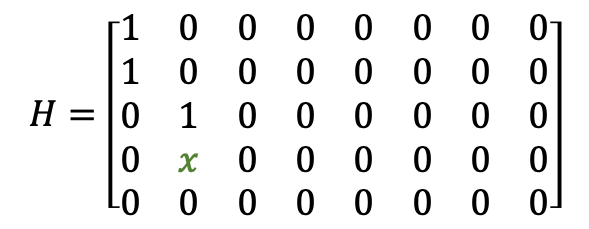
\includegraphics[scale=0.5]{pics/step4}
%	\centering 
%\end{figure}

\begin{equation}
\mathbf{H}=
\begin{tikzpicture}[baseline=-\the\dimexpr\fontdimen22\textfont2\relax ]
\matrix (m)[matrix of math nodes,left delimiter=(,right delimiter=)]
{
	1 & 0 & 0 & 0 & 0 & 0 & 0 & 0\\
	1 & 0 & 0 & 0 & 0 & 0 & 0 & 0\\
	0 & 1 & 0 & 0 & 0 & 0 & 0 & 0\\
	0 & \color{blue}x & 0 & 0 & 0 & 0 & 0 & 0\\
	0 & 0 & 0 & 0 & 0 & 0 & 0 & 0 \\
};
\begin{pgfonlayer}{myback}
%\fhighlight[green!30]{m-3-1}{m-3-8}
\end{pgfonlayer}
\end{tikzpicture}
\end{equation}

\begin{itemize}
	\item[4.] Simbol $x$ adalah calon letak elemen 1, $x$ dipilih berdasarkan baris yang memiliki nilai CND terendah. Kemudian langkah berikutnya menggunakan algoritma \textit{Anti Girth}-4, melakukan pengeceken ke kiri apabila tidak ada elemen satu maka letak tersebut akan menjadi elemen 1.
\end{itemize}

%\begin{figure}
%	\centering 
%	\hspace{1.6cm}
%	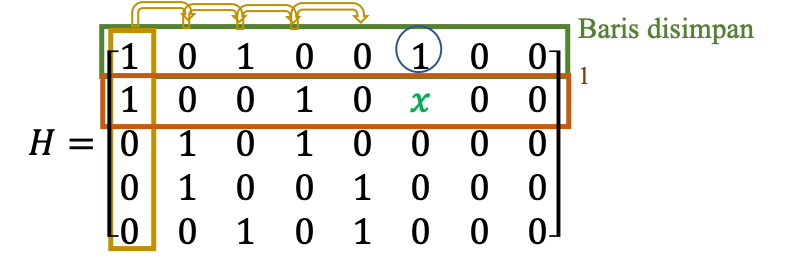
\includegraphics[scale=0.5]{pics/step5}
%	\centering 
%\end{figure}

\begin{equation}
\mathbf{H}=
\begin{tikzpicture}[baseline=-\the\dimexpr\fontdimen22\textfont2\relax ]
\matrix (m)[matrix of math nodes,left delimiter=(,right delimiter=)]
{
	1 & 0 & 1 & 0 & 0 & 1 & 0 & 0\\
	1 & 0 & 0 & 1 & 0 & \color{blue}x & 0 & 0\\
	0 & 1 & 0 & 1 & 0 & 0 & 0 & 0\\
	0 & 1 & 0 & 0 & 1 & 0 & 0 & 0\\
	0 & 0 & 1 & 0 & 1 & 0 & 0 & 0 \\
};
\begin{pgfonlayer}{myback}
\fhighlight[green!30]{m-2-1}{m-2-8}
\fhighlight[red!30]{m-1-1}{m-5-1}
\fhighlight[yellow!30]{m-1-6}{m-1-6}
\end{pgfonlayer}
\end{tikzpicture}
\end{equation}

\begin{itemize}
	\item[5.] Algoritma \textit{Anti Girth}-4 dimulai dengan menyimpan, baris dari elemen 1 sebelumnya yang nantinya akan digunakan pada pengecekan akhir. Kemudian melakukan pengecekan dari kiri ke kanan apabila ditemukan elemen 1, maka akan berlanjut ke langkah berikutnya. Apabila tidak ditemukan elemen 1 pada kolom tersebut, maka $x$ akan menjadi elemen 1. Pengecekan akan dilakukan sampai kolom sebelum kolom $x$.
\end{itemize}

%\begin{figure}
%	\centering 
%	\hspace{-1.2cm}
%	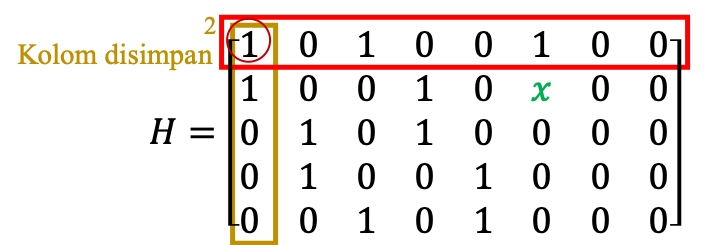
\includegraphics[scale=0.5]{pics/step6}
%	\centering 
%\end{figure}

\begin{equation}
\mathbf{H}=
\begin{tikzpicture}[baseline=-\the\dimexpr\fontdimen22\textfont2\relax ]
\matrix (m)[matrix of math nodes,left delimiter=(,right delimiter=)]
{
	1 & 0 & 1 & 0 & 0 & 1 & 0 & 0\\
	1 & 0 & 0 & 1 & 0 & \color{blue}x & 0 & 0\\
	0 & 1 & 0 & 1 & 0 & 0 & 0 & 0\\
	0 & 1 & 0 & 0 & 1 & 0 & 0 & 0\\
	0 & 0 & 1 & 0 & 1 & 0 & 0 & 0 \\
};
\begin{pgfonlayer}{myback}
\fhighlight[green!30]{m-1-1}{m-1-8}
\fhighlight[red!30]{m-1-1}{m-5-1}
\fhighlight[yellow!30]{m-1-1}{m-1-1}
\end{pgfonlayer}
\end{tikzpicture}
\end{equation}

\begin{itemize}
	\item[6.] Langkah ke-2 Algoritma \textit{Anti Girth}-4, menyimpan kolom dari elemen 1 yang ditemukan pada proses pengecekan di langkah pertama. 
	\item [7.] Kemudian melakukan pengecekan akhir, yaitu apabila
	\begin{equation}
	\mathbf{H}_{Baris\_simpan, Kolom\_simpan}=1,
	\end{equation}
	pada $x$ akan terbentuk \textit{girth} 4 jika $x$ berelemen 1, sehingga $x$ akan berpindah ke \textit{check node} dengan CND minimal berikutnya dan melakukan pengecekan lagi.
\end{itemize}

Matriks \textit{parity check} LDPC \textit{codes} yang terbentuk dan graf pohon pada variable \textit{nodes} ke-dua menggunakan aturan PEG ditunjukkan oleh Gambar \ref{fig:PEGM}. Dapat diketahui bahwa matriks \textit{parity check} tidak menghasilkan \textit{girth}-4.
\begin{figure}[tb]
	\centering 
	\hspace{-1.2cm}
	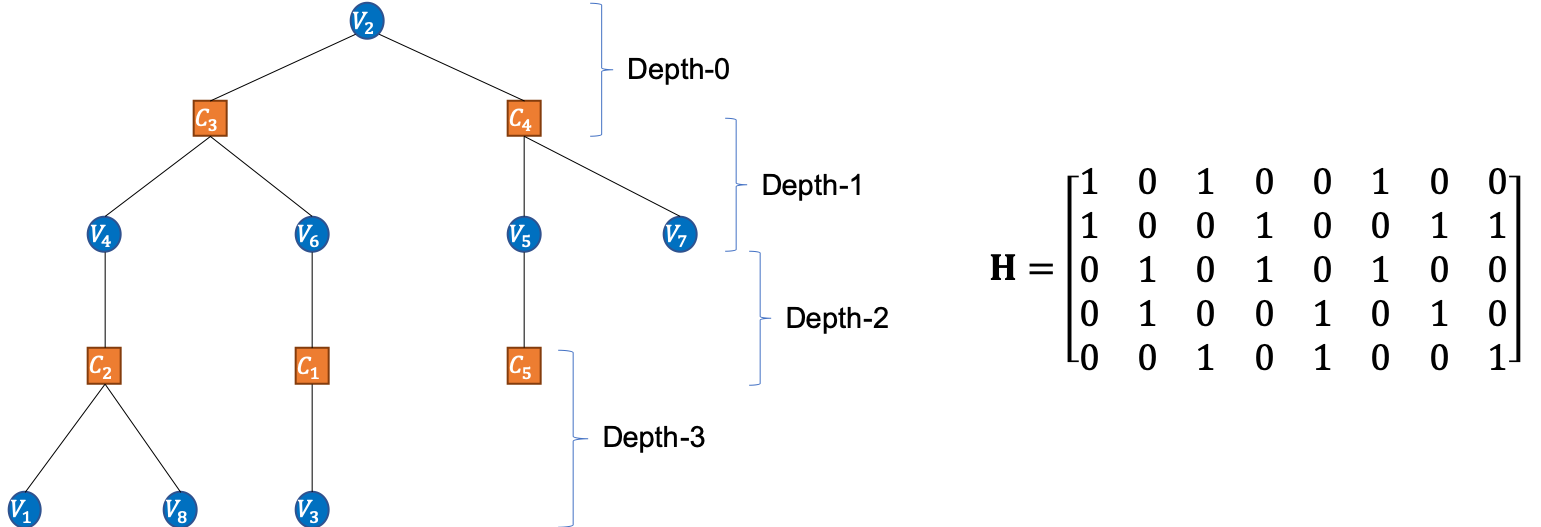
\includegraphics[width=1\textwidth]{pics/withmatlabpeg2}
	\centering 
	\caption{Hasil graf pohon dan matriks \textit{parity check} LDPC \textit{codes} menggunakan algoritma PEG yang diusulkan.}
	\label{fig:PEGM}
\end{figure}

\subsection{Usulan LDPC \textit{Codes} DVB-T2 menggunakan PEG}
Tugas Akhir ini juga mengusulkan \textit{degree distribution} untuk \textit{downscaled} LDPC \textit{codes} DVB-T2 dengan menggunakan algoritma PEG. \textit{Degree distribution} pada \textit{downscaled} LDPC \textit{codes} yang diusulkan untuk \textit{code rate} $R_e=\frac{4}{9}$ adalah:
\begin{eqnarray}
\Lambda (x) &=& \frac{1}{270}x+\frac{149}{270}x^2+\frac{90}{270}x^3+\frac{30}{270}x^8 \\
\Omega(x) &=& \frac{92}{150}x^5+\frac{58}{150}x^6,
\end{eqnarray}
untuk \textit{code rate} $R_e=\frac{3}{5}$ adalah:
\begin{eqnarray}
\Lambda (x) &=& \frac{1}{270}x+\frac{107}{270}x^2+\frac{132}{270}x^3+\frac{1}{270}x^7+\frac{7}{270}x^8 \nonumber \\ &&+\frac{1}{270}x^9+\frac{11}{270}x^{10}+\frac{10}{270}x^{12},   \\
\Omega(x) &=& \frac{59}{108}x^8+\frac{49}{108}x^9,
\end{eqnarray}
untuk \textit{code rate} $R_e=\frac{2}{3}$ adalah:
\begin{eqnarray}
\Lambda (x) &=& \frac{1}{270}x+\frac{89}{270}x^2+\frac{162}{270}x^3+\frac{1}{270}x^7 \nonumber \\ &&+\frac{9}{270}x^8+\frac{1}{270}x^{12}+\frac{7}{270}x^{13} ,  \\
\Omega(x) &=& \frac{37}{90}x^{10}+\frac{53}{90}x^9,
\end{eqnarray}
untuk \textit{code rate} $R_e=\frac{11}{15}$ adalah:
\begin{eqnarray}
\Lambda (x) &=& \frac{1}{270}x+\frac{71}{270}x^2+\frac{192}{270}x^3+\frac{6}{270}x^{12},   \\
\Omega(x) &=& \frac{4}{72}x^{10}+\frac{65}{72}x^{11},+\frac{3}{72}x^{12},
\end{eqnarray}
untuk \textit{code rate} $R_e=\frac{7}{9}$ adalah:
\begin{eqnarray}
\Lambda (x) &=& \frac{1}{270}x+\frac{59}{270}x^2+\frac{210}{270}x^3,  \\
\Omega(x) &=& \frac{31}{60}x^{12}+\frac{29}{60}x^{13},
\end{eqnarray}
untuk \textit{code rate} $R_e=\frac{37}{45}$ adalah:
\begin{eqnarray}
\Lambda (x) &=& \frac{1}{270}x+\frac{76}{270}x^2+\frac{185}{270}x^3 +\frac{2}{270}x^4+\frac{1}{270}x^{12}+\frac{3}{270}x^{13},  \\
\Omega(x) &=& \frac{5}{48}x^{15}+\frac{39}{48}x^{16}+\frac{2}{48}x^{17}+\frac{2}{48}x^{18}.
\end{eqnarray}


%\subsection{\textit{Formatting} Tulisan}
%\begin{itemize}
%\item Tulisan Tebal (\textit{Bold})\\
%\textbackslash textbf\{\textit{argument}\} untuk menebalkan tulisan.\\
%contoh:
%\textbackslash textbf\{tulisan tebal\} $\rightarrow$ \textbf{tulisan tebal}
%
%\item Tulisan Miring (\textit{Italic})\\
%\textbackslash textit\{\textit{argument}\} untuk memiringkan tulisan.\\
%contoh:
%\textbackslash textit\{tulisan miring\} $\rightarrow$ \textit{tulisan miring}
%
%\item Tulisan Bergaris Bawah (\textit{Underlined})\\
%\textbackslash uline\{\textit{argument}\} untuk menggarisbahwahi tulisan.\\
%contoh:
%\textbackslash uline\{tulisan bergaris bawah\} $\rightarrow$ \uline{tulisan bergaris bawah}
%
%\item Tulisan Menggantung ke Atas (\textit{Superscript})\\
%\textbackslash textsuperscript\{\textit{argument}\} untuk membuat tulisan menggantung.\\
%contoh:
%\textbackslash textsuperscript\{tulisan menggantung\} $\rightarrow$ \textsuperscript{tulisan menggantung ke atas}
%
%\item Tulisan Menggantung ke Bawah (\textit{Subscript})\\
%\textbackslash textsubscript\{\textit{argument}\} untuk membuat tulisan menggantung.\\
%contoh:
%\textbackslash textsubscript\{tulisan menggantung\} $\rightarrow$ \textsubscript{tulisan menggantung ke bawah}
%
%\item Tulisan yang Dicoret (\textit{Strike-through})
%\textbackslash sout\{\textit{argument}\} untuk membuat tulisan tercoret.\\
%contoh:
%\textbackslash sout\{tulisan tercoret\} $\rightarrow$ \sout{tulisan tercoret}
%\end{itemize}
%
%\subsection{Memasukkan Gambar}
%Untuk memasukkan gambar ke dalam dokumen, digunakan \textit{syntax} \textbackslash begin\{figure\} ... \textbackslash end\{figure\}. Berikut contoh memasukkan \textit{file} gambar \textit{bipartite.png} yang berada di dalam folder \textit{pics/diagram/}. Dari kode tersebut didapatkan hasil gambar \ref{fig:bipartite}. Label dapat diberikan di dalam \textit{figure}, sehingga untuk merujuk sebuah gambar dapat digunakan \textit{ref}. Contoh penggunaan \textit{ref}, misalkan \textbackslash ref\{fig:bipartite\} $\rightarrow$ \ref{fig:bipartite}.
%
%\begin{lstlisting}
%\begin{figure}
%	\centering
%	\includegraphics[width=0.6\textwidth]
%		{pics/diagram/bipartite.png}
%		\caption{Topologi \textit{Bipartite} untuk Pengukuran Fail-Over Delay}
%	\label{fig:bipartite}
%\end{figure}
%\end{lstlisting}
%
%\begin{figure}
%	\centering
%	\includegraphics[width=0.6\textwidth]
%		{pics/diagram/bipartite.png}
%		\caption{Topologi \textit{Bipartite} untuk Pengukuran Fail-Over Delay}
%	\label{fig:bipartite}
%\end{figure}
%
%\subsection{Membuat Tabel}
%Untuk memasukkan tabel ke dalam dokumen, digunakan \textit{syntax} \textbackslash begin\{table\} ... \textbackslash end\{table\}
%
%\begin{lstlisting}
%\begin{table}
%	\centering
%	\caption{Jumlah \textit{Switch} dan \textit{Host} serta Jenis \textit{Traffic} untuk Setiap Pengukuran}
%	\label{tab:tab1}
%	\begin{tabular}{| l | r | r | r | c |}
%		\hline
%		Pengukuran & L1 & L2 & \textit{Host} & \textit{Traffic}\\ 
%		\hline
%		\textit{Fail-Over Delay} & 2 - 4  & 1 - 8 & 1 - 8 & ICMP Ping Tunggal\\
%		\textit{Load Balance: Load Distribution} & 1 - 4 & 1 & 1 & 200 UDP \textit{Flows}\\
%		\textit{Load Balance: Performance} & 1 - 4  & 1 - 8 & 1 - 8 & Data, Video, VoIP \textit{Flows}\\
%		\textit{Overhead Size} & 2 & 1 & 1 & 25 - 150 UDP \textit{Flows}\\
%		\textit{Memory Consumption: Switch} & 1 - 4  & 1 - 8 & 0 & -\\
%		\textit{Memory Consumption: Host}  & 1 & 1 & 0 - 200 & - \\
%		\hline
%	\end{tabular}
%\end{table}
%\end{lstlisting}
%
%\begin{table}
%	\centering
%	\caption{Jumlah \textit{Switch} dan \textit{Host} serta Jenis \textit{Traffic} untuk Setiap Pengukuran}
%	\label{tab:tab1}
%	\begin{tabular}{| l | r | r | r | c |}
%		\hline
%		Pengukuran & L1 & L2 & \textit{Host} & \textit{Traffic}\\ 
%		\hline
%		\textit{Fail-Over Delay} & 2 - 4  & 1 - 8 & 1 - 8 & ICMP Ping Tunggal\\
%		\textit{Load Balance: Load Distribution} & 1 - 4 & 1 & 1 & 200 UDP \textit{Flows}\\
%		\textit{Load Balance: Performance} & 1 - 4  & 1 - 8 & 1 - 8 & Data, Video, VoIP \textit{Flows}\\
%		\textit{Overhead Size} & 2 & 1 & 1 & 25 - 150 UDP \textit{Flows}\\
%		\textit{Memory Consumption: Switch} & 1 - 4  & 1 - 8 & 0 & -\\
%		\textit{Memory Consumption: Host}  & 1 & 1 & 0 - 200 & - \\
%		\hline
%	\end{tabular}
%\end{table}
%
%\subsection{Notasi Matematika}
%Untuk menuliskan notasi matematika, pada \latex digunakan \textit{syntax} \$ ... \$ untuk penggunaan di dalam paragraf dan \textbackslash begin\{equation\} ... \textbackslash end\{equation\} untuk penggunaan terpisah di luar paragraf. Sebagai contoh sebagai berikut.
%\begin{itemize}
%\item contoh 1:
%\begin{lstlisting}
%\begin{equation}
%	metric_{i,j} = \frac{10^2}{(capacity_{E_{i,j}} - 	load_{E_{i,j}})}
%	\label{eq:metric1}
%\end{equation}
%\end{lstlisting}
%\begin{equation}
%	metric_{i,j} = \frac{10^2}{(capacity_{E_{i,j}} - 	load_{E_{i,j}})}
%	\label{eq:metric1}
%\end{equation}
%\item contoh 2:
%\begin{lstlisting}
%\begin{equation}
%	f(x)=(x+a)(x+b)
%	\label{eq:fx1}
%\end{equation}
%\end{lstlisting}
%\begin{equation}
%	f(x)=(x+a)(x+b)
%	\label{eq:fx1}
%\end{equation}
%\item contoh 3
%\begin{lstlisting}
%\begin{subequations}
%Maxwell's equations:
%	\begin{align}
%		B'&=-\nabla \times E,\\
%		E'&=\nabla \times B - 4\pi j,
%	\end{align}
%	\label{eq:maxwell}
%\end{subequations}
%\end{lstlisting}
%\begin{subequations}
%Maxwell's equations:
%	\begin{align}
%		B'&=-\nabla \times E,\\
%		E'&=\nabla \times B - 4\pi j,
%	\end{align}
%	\label{eq:maxwell}
%\end{subequations}
%\item contoh 4
%\begin{lstlisting}[language=tex]
%matriks $Adj$ digunakan untuk menggambarkan topologi jaringan  $G = (V,E)$, di mana $V = \{v_{1}, v_{2}, ..., v_{n}\}$ merupakan \textit{switch} dan $E = \{e_{1,1}, e_{1,2}, ..., e_{n,n}\}$ merupakan \textit{link} antar-\textit{switch}. Setiap $E_{i,j}$ menyimpan informasi \textit{metric} sesuai persamaan \ref{eq:metric1} . Hasil dari algoritma ini adalah jalur $T_{k,l}$ yang disimpan di dalam \textit{bucket Path} atau $T$. Setiap $T_{k,l}$ mempunyai nilai \textit{metric} sesuai persamaan \ref{eq:metric2}.
%\end{lstlisting}
%matriks $Adj$ digunakan untuk menggambarkan topologi jaringan  $G = (V,E)$, di mana $V = \{v_{1}, v_{2}, ..., v_{n}\}$ merupakan \textit{switch} dan $E = \{e_{1,1}, e_{1,2}, ..., e_{n,n}\}$ merupakan \textit{link} antar-\textit{switch}. Setiap $E_{i,j}$ menyimpan informasi \textit{metric} sesuai persamaan \ref{eq:metric1}. Hasil dari algoritma ini adalah jalur $T_{k,l}$ yang disimpan di dalam \textit{bucket Path} atau $T$. Setiap $T_{k,l}$ mempunyai nilai \textit{metric} sesuai persamaan 3.2.
%\end{itemize} 
%
%\subsection{Notasi Algoritma \textit{Pseudo-Code}}
%Untuk menuliskan \textit{pseudo-code} digunakan \textit{syntax} \textbackslash begin\{algorithm\} ... \textbackslash end\{algorithm\}. Berikut contoh notasi \textit{pseudo code}.
%\begin{lstlisting}
%\begin{algorithm}
%\caption{--- Find all possible path from graph G --- Adapted from DFS algorithm}\label{alg1}
%\begin{algorithmic}[1]
%\Require network topology $G = (V,E)$ represented in dictionary $Adj$, where $V, E$ represents DPID and link between DPID
%\Ensure a routing table for source-destination DPID pairs represented in dictionary $T$
%\State $T \leftarrow \{\}$
%\Procedure{Per\textunderscore Source\textunderscore DFS}{$source, origin =$ None, $path \leftarrow []$}
%  \If{$origin \equiv$ None}
%    \State $origin \leftarrow source$
%  \EndIf
%  \For{$i \in M[source]$}
%    \If{$i \in path \lor i \equiv origin$}
%      \State continue
%    \Else
%      \If{$i \notin T[origin]$}
%        \State $T[origin][i] \leftarrow [path + [i])]$
%        \Else
%          \State append $[path + [i])]$ to $T[origin][i]$
%      \EndIf
%      \State PER\textunderscore SOURCE\textunderscore DFS($i, origin, path + [i]$)
%    \EndIf
%  \EndFor
%\EndProcedure
%\For{$i \in Adj$}
%  \State $path[i] \leftarrow \{\}$
%  \State PER\textunderscore SOURCE\textunderscore DFS($i$)
%\EndFor
%\end{algorithmic}
%\end{algorithm}
%\end{lstlisting}
%
%\begin{algorithm}
%\caption{--- Find all possible path from graph G --- Adapted from DFS algorithm}\label{alg1}
%\begin{algorithmic}[1]
%\Require network topology $G = (V,E)$ represented in dictionary $Adj$, where $V, E$ represents DPID and link between DPID
%\Ensure a routing table for source-destination DPID pairs represented in dictionary $T$
%\State $T \leftarrow \{\}$
%\Procedure{Per\textunderscore Source\textunderscore DFS}{$source, origin =$ None, $path \leftarrow []$}
%  \If{$origin \equiv$ None}
%    \State $origin \leftarrow source$
%  \EndIf
%  \For{$i \in M[source]$}
%    \If{$i \in path \lor i \equiv origin$}
%      \State continue
%    \Else
%      \If{$i \notin T[origin]$}
%        \State $T[origin][i] \leftarrow [path + [i])]$
%        \Else
%          \State append $[path + [i])]$ to $T[origin][i]$
%      \EndIf
%      \State PER\textunderscore SOURCE\textunderscore DFS($i, origin, path + [i]$)
%    \EndIf
%  \EndFor
%\EndProcedure
%\For{$i \in Adj$}
%  \State $path[i] \leftarrow \{\}$
%  \State PER\textunderscore SOURCE\textunderscore DFS($i$)
%\EndFor
%\end{algorithmic}
%\end{algorithm}
%
%\subsection{Penulisan Daftar Referensi}
%Terdapat banyak sekali gaya penulisan daftar referensi. Pada \textit{template} ini penulisan daftar referensi merujuk ke IEEE. Gaya penulisan daftar referensi IEEE \cite{ieee_style} memiliki beberapa format yang berbeda untuk jenis referensi yang berbeda. Jenis-jenis publikasi yang diterangkan cara penulisan daftar referensinya oleh IEEE antara lain: \textit{paper} jurnal, \textit{paper} seminar/\textit{conference}, dokumen paten, dokumen standar, dokumen laporan/\textit{report}, tesis dan disertasi, buku, serta beberapa dokumen, artikel, perangkat lunak, maupun sumber kode yang tersedia \textit{online}. Pada \textit{pustaka.tex}, sudah dibuat beberapa daftar referensi sebagai contoh dalam pembuatan daftar referensi lain yang diinginkan oleh penulis.


\section{Usulan Teknik untuk Menghitung \textit{Girth} LDPC \textit{Codes}}
		\begin{figure}[tb]
	\centering 
	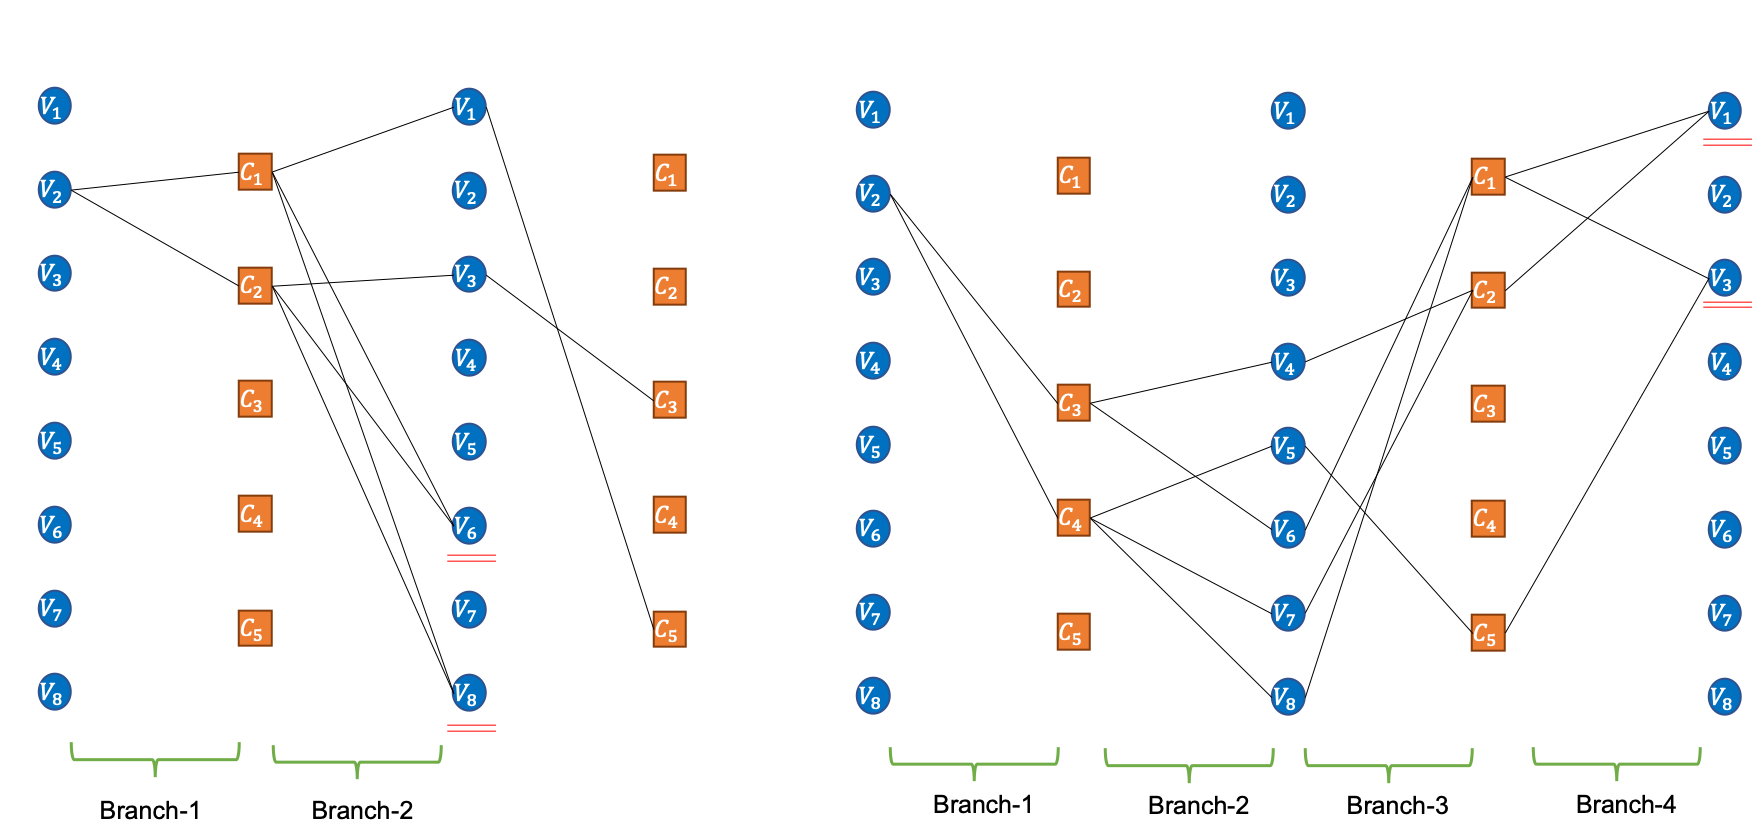
\includegraphics[width=1\textwidth]{pics/hitunggirth}
	\centering 
	\caption{Algoritma untuk menghitung \textit{girth} LDPC \textit{codes} yang diusulkan.}
	\label{fig:girthhitung}
\end{figure}
Tugas Akhir ini mengusulkan sebuah teknik untuk menghitung \textit{girth} dari setiap \textit{variable nodes} pada LDPC \textit{codes}, sehingga dapat diketahui distribusi \textit{local girth} dari LDPC \textit{codes}. \textit{Girth} adalah nilai \textit{local girth} terkecil dari distribusi \textit{girth} LDPC \textit{codes}. Teknik yang diusulkan adalah hasil dari modifikasi dan pengembangan dari algoritma pembuatan graf pohon pada PEG ditunjukkan oleh Gambar \ref{fig:girthhitung}. Berikut langkah-langkah untuk menghitung \textit{girth} yang diusulkan:
\begin{enumerate}
	\item Tentukan satu \textit{variable node} dan sebarkan \textit{edges}-nya sesuai dari matriks.
	\item Sebarkan \textit{edges} terus menerus sampai terdapat \textit{node} yang tidak dapat menyebarkan \textit{edge}.
	\item Hitung \textit{branch} $b$ dimulai dari satu, lalu dengan menggunakan persamaan
	\begin{equation}
	g=b\times 2,
	\end{equation}
	maka nilai \textit{local girth} $g$ dapat diketahui.
\end{enumerate}